\chapter{Coupled Multiphysics Results}
\label{ch:coupledResults}

\section{Power Reactor Modeling}
\label{sec:power_reactor_modeling}
  The motivation for this work is to model nuclear power reactors with
  multiphysics feedback. This has been accomplished by modeling the reactor
  power distribution with the multigroup neutron diffusion equation solved via
  the \gls{fem} (\chref{ch:neutronDiffusion}). Axial heat convection and radial
  heat conduction models are used to estimate reactor material temperatures
  (\chref{ch:thermalHydraulics}).  Simplified thermal expansion modeling is used
  to model reactor dimensions (\chref{ch:thermalExpansion}). Combined, these
  multiphysics effects will provide feedback which can be estimated in a
  realistic core model.
  
  To test the coupling of these models, a realistic reactor benchmark is
  provided and modeled in \sref{sec:abr}. Reactivity coefficients describing 
  system feedback are defined in \sref{sec:reactivity_coefficients}. Results are
  presented in \sref{sec:results}.

\section{\glsentrylong{abr} -- MET-1000}
\label{sec:abr}
  The \gls{abr} is a benchmark reactor design is proposed by \gls{oecd}
  \gls{nea} \cite{abr}. The \gls{abr} is fueled with a ternary alloy metallic
  fuel and has a 1,000 \units{MWth} rating; hence, MET-1000. This is a
  medium-sized, metallic-fueled reactor with a total of 180 hexagonal assemblies
  and is 4.8 \units{m} tall.  The benchmark is fully specified and 31
  independent results have been submitted so far. Compared to other benchmark
  problems modeled in this thesis, this model is extremely large due to the
  large structural components included above and below the active fuel region.
  
  Each submission to the benchmark uses independently generated cross sections
  from several different cross section libraries (e.g. ENDF/B-VII.0, JEFF3.1,
  etc.). Therefore, using this benchmark as a verification problem is not
  feasible. Cross sections were generated for this model using \mcc and the 
  procedure outlined in \sref{sec:cross_section_treatment}. This procedure
  resulted in temperature-dependent cross section libraries with 33 energy
  groups. 
  
  To verify the \gls{fem} model, the multigroup neutron diffusion equation is
  solved with the same cross sections using \dif and the \gls{fem}
  solution from \chref{ch:neutronDiffusion}. In this verification, cross
  sections are fixed at the value associated with nominal reactor temperatures
  and multiphysics feedback is disabled, as \dif has no multiphysics
  capabilities. \dif and the \gls{fem}, using the same cross sections, agree to
  692 \units{\glsentryshort{\glsentryshort{pcm}}}. The \dif and \gls{fem}
  models were minimally refined. Initially, an unrefined geometry was modeled
  with six triangles per hexagon and 80 axial elevations, implying a wedge
  height of $6~\units{cm}$. This unrefined model had a total of 30,320 elements.
  The model was then spatially refined with 24 triangles per hexagon and 160
  axial elevations, implying a wedge height of $3~\units{cm}$. The once refined
  model had a total of 242,560 elements. Results from this brief verification
  study are presented in \tref{tab:abr_benchmark}. A more formal mesh refinement
  study would presumably show further error reduction. 

  \begin{table}
    \begin{center}
      \caption{\glsentrylong{abr} Refinement Results.}
      \label{tab:abr_benchmark}
      \begin{tabular}{cccc}
        \toprule
        Refinement & \dif $\keff$ & \gls{fem} $\keff$ & Difference
          \units{\glsentryshort{pcm}}\\
        \midrule
        0 & 1.017906 & 0.999339 & 1856.7 \\
        1 & 1.013614 & 1.006694 & 692.0 \\
        \bottomrule
      \end{tabular}
    \end{center}
  \end{table}
  
  Reactor materials in the benchmark are shown in \fref{fig:abr_materials}.
  For the sole purpose of intuitive flux visualization, the 33-group energy
  structure is collapsed to a two-group energy structure. The collapsed fast
  ($\phi_1$) and collapsed thermal ($\phi_2$) are plotted in
  \fref{fig:abr_fluxes}. Note: all subsequent results presented are generated
  with the full 33-group energy structure. Fast flux is shown to peak in the
  center of the core in the active fuel region. Thermal flux is shown to peak
  in core structural material, at the periphery of the active fuel region, as
  well as in control rod locations where the control rods have been withdrawn
  from the active fuel region.

  \begin{figure}
    \centering
    
\includegraphics[width=0.4\textwidth]{abr_materials}
    \caption{Materials in \glsentryshort{abr}.}
    \label{fig:abr_materials}
  \end{figure}

  \begin{figure}
    \centering
    \subfloat[$\phi_{1}$]{
      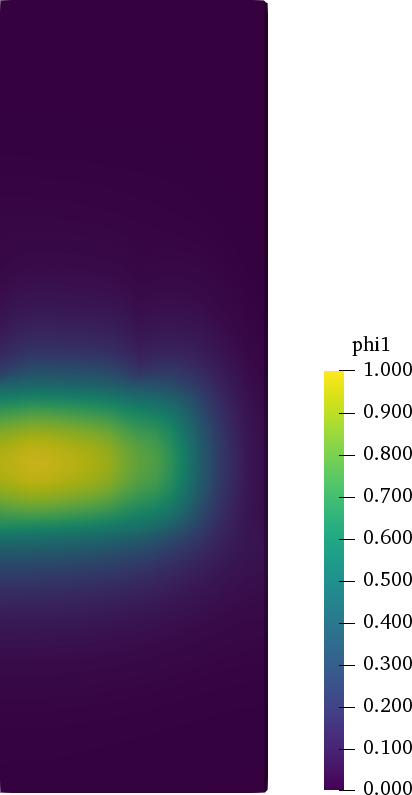
\includegraphics[width=0.25\textwidth]{abr_phi_nod_group1}}
    \hspace{0.2in}
    \subfloat[$\phi_{2}$]{
      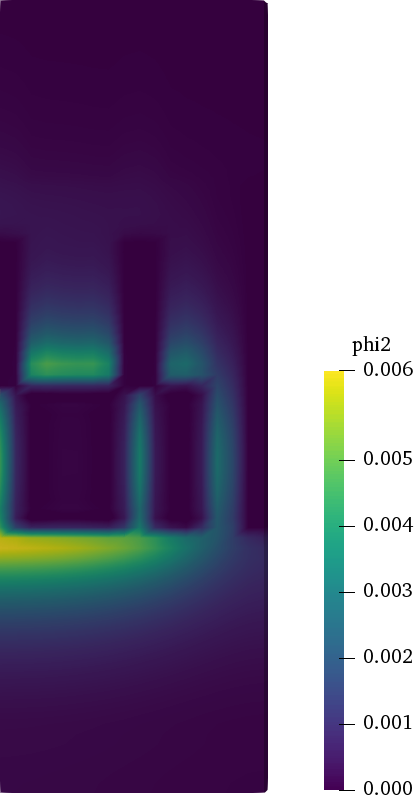
\includegraphics[width=0.25\textwidth]{abr_phi_nod_group2}}
    \caption{Fast and Thermal Neutron Flux in \glsentryshort{abr}.}
    \label{fig:abr_fluxes}
  \end{figure}

  Multiphysics results for this benchmark have not been published. Therefore,
  the coupled results are not compared to reference results. Instead, each of
  the multiphysics models has been investigated individually in the preceding
  chapters. 

\section{Reactivity Coefficients}
\label{sec:reactivity_coefficients}
  Reactivity of a reactor can be used to compare the state of the reactor to the
  critical state. Reactivity $\rho$ is defined as
  \begin{equation}
    \label{eq:reactivity}
    \rho \units{\glsentryshort{pcm}} = \frac{\keff-1}{\keff} \times 10^5.
  \end{equation}
  Recall $\keff < 1$ for a subcritical reactor, $\keff=1$ for a critical
  reactor, and $\keff > 1$ for a supercritical reactor. Therefore $\rho < 0$
  for a subcritical reactor, $\rho = 0$ for a critical reactor, and $\rho > 0$
  for a supercritical reactor. 

  A reactivity coefficient can be defined as a partial derivative with respect
  to a quantity of interest \cite{textbookknief}. Let $\alpha_x$ be the 
  reactivity coefficient for quantity $x$, then
  \begin{equation}
    \label{eq:reactivity_coefficient}
    \alpha_x(x_i) = \left. \frac{\partial \rho}{\partial x} \right|_{x=x_i}
  \end{equation}
  where $\rho$ is the reactivity defined by \eref{eq:reactivity}.
  \eref{eq:reactivity_coefficient} is useful for estimating reactor dynamics.
  For some change in reactor state $\Delta x$, the reactivity response can be
  estimated as 
  \begin{equation}
    \label{eq:reactivity_estimate}
    \Delta \rho \approx \alpha_x(x_i) \, \Delta x.
  \end{equation}
  It is expected that reactivity coefficients will vary as reactor conditions
  vary. Therefore, it will be necessary to calculate $\alpha_x$ as a function of
  reactor condition $x_i$. Specifically, reactor power, $Q_{Rx}$, will be varied 
  in the calculation of $\alpha$. Therefore, a set of reactor powers varying 
  from $0\%$ to $100\%$ as $Q_{Rx,i} = \{0\%,\ldots,100\%\}$ will be used.

  Reactivity coefficients useful for fast reactor applications include the power
  coefficient, thermal expansion coefficient, fuel temperature (Doppler)
  coefficient, and \gls{ctc} \cite{textbookknief}.  Reactivity coefficients will
  be estimated with a first-order, forward-Euler, finite-difference
  approximation such that
  \begin{equation}
    \label{eq:reactivity_coefficient_finite_difference}
    \alpha_x(x_i) \approx \frac{\rho(x_i) - \rho(x_i + \Delta x)}{\Delta x}
  \end{equation}
  for a given $\Delta x$. The evaluation of
  \eref{eq:reactivity_coefficient_finite_difference} is discussed in the
  following sections for relevant reactivity coefficients.

  \subsection{Power Reactivity Coefficient}
  \label{sec:power_reactivity_coefficient}
    The power reactivity coefficient measures the reactivity response due to a
    power increase. In a stable reactor, $\alpha_{power} < 0$ to ensure an
    increase in reactor power requires a reactivity increase and to prevent a
    runaway power increase. To evaluate $\alpha_{power}$, the reactor is
    simulated at a nominal reactor power, $Q_{Rx,i}$ resulting in
    $\keff(Q_{Rx,i})$. Then, reactor power is increased by $\Delta Q_{Rx}$
    resulting in $\keff(Q_{Rx,i} + \Delta Q_{Rx})$. These $\keff$ values
    correspond to reactivities $\rho(Q_{Rx,i})$ and ${\rho(Q_{Rx,i} + \Delta
    Q_{Rx})}$ respectively as defined by \eref{eq:reactivity}. With these
    values, the power reactivity coefficient can be calculate as
    \begin{equation}
      \label{eq:power_reactivity_coefficient}
      \alpha_{power}(Q_{Rx,i}) = \frac{\rho(Q_{Rx,i}) - \rho(Q_{Rx,i} + 
        \Delta Q_{Rx})} {\Delta Q_{Rx}}.
    \end{equation}
    A typical value of $\Delta Q_{Rx}$ is $5\% Q_{Rx}$.

  \subsection{Thermal Expansion Reactivity Coefficient}
  \label{sec:thermal_expansion_reactivity_coefficent}
    The thermal expansion reactivity coefficient describes the reactivity 
    response due solely to thermal expansion for a given increase in reactor 
    power. It is expected that thermal expansion will be the dominant 
    contribution to the power reactivity coefficient in fast reactors. This is 
    due to two main reasons: the significant thermal expansion of metal fuels at
    high temperature  and the large neutron leakage fraction ($\leakage \approx
    20\%$) in fast reactors (see \chref{ch:thermalExpansion}).

    Thermal expansion temperatures, \texpfuel and \texpstruct, as implemented in
    \chref{ch:thermalExpansion} must be known before the simulation. Note from
    \sref{sec:power_reactivity_coefficient}, a case must be simulated to
    calculate $\keff(Q_{Rx_i} + \Delta Q_{Rx})$ in the calculation of the power
    reactivity coefficient in \eref{eq:power_reactivity_coefficient}. Therefore, 
    the temperature distribution resulting from this study can be used to
    calculate the thermal expansion temperatures for the case with increased
    power, ${\texp(Q_{Rx,i} + \Delta Q_{Rx})}$. Then, the thermal expansion
    reactivity coefficient is 
    \begin{equation}
      \label{eq:thermal_expansion_reactivity_coefficient}
      \alpha_{thexp}(Q_{Rx,i}) = \frac{\rho(\texp(Q_{Rx,i})) - 
        \rho(\texp(Q_{Rx,i} + \Delta Q_{Rx}))}
        {\Delta Q_{Rx}}
    \end{equation}
    where $\texp(Q_{Rx,i})$ represents the thermal expansion temperatures for
    power $Q_{Rx,i}$ and $\texp(Q_{Rx,i} + \Delta Q_{Rx})$ represents the
    thermal expansion temperatures for power $Q_{Rx,i} + \Delta Q_{Rx}$. Note
    that in \eref{eq:thermal_expansion_reactivity_coefficient}, only thermal
    expansion temperatures are changed, not the true reactor power $Q_{Rx}$.
    A typical value of $\Delta Q_{Rx}$ is $5\% Q_{Rx}$.

  \subsection{Fuel Temperature Reactivity Coefficient}
  \label{sec:fuel_temperature_reactivity_coefficient}
    The fuel temperature reactivity coefficient measures the reactivity change 
    due to an increase in fuel temperature. This coefficient is often termed the
    Doppler coefficient because the reactivity effect is due to the Doppler
    broadening of resonance absorption peaks in heavy nuclei such as
    \isotope[238]{U} \cite{textbookknief}. Briefly, at high fuel temperatures, 
    neutrons are more likely to be parasitically absorbed by non-fissile nuclei
    than fissile nuclei in the fuel material.

    To calculate $\alpha_{Doppler}$, fuel temperature is increased directly. A
    simulation is conducted with feedback for reactor power $Q_{Rx,i}$ and the
    temperature profile is stored. Then, the fuel temperature is uniformly 
    increased in the reactor by $\Delta T_{fuel}$ and the simulation is
    conducted again. This procedure will result in $\keff(Q_{Rx,i})$ and
    ${\keff(T_{fuel} + \Delta T_{fuel})}$. Then, the Doppler reactivity 
    coefficient follows.
    \begin{equation}
      \label{eq:doppler_reactivity_coefficient}
      \alpha_{Doppler}(Q_{Rx,i}) = \frac{\rho(Q_{Rx,i}) - \rho_i(T_{fuel} +
        \Delta T_{fuel})} {\Delta T_{fuel}}
    \end{equation}
    Note that the Doppler reactivity coefficient is always negative. A typical
    value of $\Delta T_{fuel}$ is $5~\units{K}$. The definition in
    \eref{eq:doppler_reactivity_coefficient} is a \textit{uniform} Doppler
    coefficient as opposed to a \textit{distributed} Doppler coefficient because
    temperatures are increased uniformly throughout the reactor.

  \subsection{\texorpdfstring{\glsentrylong{ctc}}{Coolant Temperature
    Coefficient (CTC)}}
  \label{sec:coolant_temperature_reactivity_coefficient}
    The \gls{ctc} describes the reactivity change due to an increase in coolant
    temperature. In \glspl{lwr}, this may be called the \gls{mtc} but in fast
    reactors, the coolant is not designed to moderate neutrons. Feedback in the
    coolant is due to two main phenomena: the decrease in absorption cross
    sections in the coolant due to Doppler broadening and the decrease of
    density due to temperature increase. The dominant effect is the decrease of
    sodium density due to the temperature increase \cite{textbookknief}.

    Unlike all other reactivity coefficients presented here, the \gls{ctc} of
    the \gls{abr} is positive as is common in fast reactors. This implies an
    increase in coolant temperature will lead to an increase in reactivity and
    cause a subsequent increase in reactor power. In fast reactors, the coolant
    acts as a parasitic neutron absorber. Therefore, a decrease in the sodium
    absorption cross section or a decrease in sodium density due to a
    temperature increase encourages neutron absorption in fissile material in
    the fuel and results in a reactivity increase. This does not pose a 
    stability problem as long as the power reactivity coefficient remains 
    negative.

    To calculate $\alpha_{CTC}$, coolant temperature is increased directly with
    a procedure similar to that for the Doppler reactivity coefficient in
    \sref{sec:fuel_temperature_reactivity_coefficient}. A simulation is
    conducted with feedback for reactor power $Q_{Rx,i}$ and the temperature
    profile is stored. Then, the coolant temperature is uniformly increased by
    $\Delta T_{cool}$ and the simulation is conducted again. This procedure will
    result in $\keff(Q_{Rx,i})$ and ${\keff(T_{cool} + \Delta T_{cool})}$. Then,
    the \gls{ctc} follows.
    \begin{equation}
      \label{eq:coolant_temperature_reactivity_coefficient}
      \alpha_{CTC}(Q_{Rx,i}) = \frac{\rho(Q_{Rx,i}) - \rho(T_{cool} + 
        \Delta T_{cool})} {\Delta T_{cool}}
    \end{equation}
    A typical value for $\Delta T_{cool}$ is $5~\units{K}$.

\section{Results}
\label{sec:results}
  Returning to the \gls{abr} MET-1000 benchmark, reactivity coefficients are
  modeled for this reactor. The methodology and formulae from
  \sref{sec:reactivity_coefficients} are used. The reactor $\keff$ as a function
  of reactor power is plotted in \fref{fig:keff_effects}. Note $\keff$ decreases
  as power increases implying a negative power coefficient.
  
  The reactivity coefficients themselves are plotted in
  \fref{fig:abr_reactivity_coefficients}. The combined power reactivity
  coefficient is plotted in \fref{fig:power_reactivity_coefficient}. Note,
  $\alpha_{power} < 0$ for all powers.  The \gls{ctc} is positive as shown in
  \fref{fig:coolant_temperature_reactivity_coefficient} and as expected.  The
  Doppler coefficient is negative as shown in
  \fref{fig:doppler_reactivity_coefficient} and as expected. The \gls{ctc}
  becomes more positive at high powers but the magnitude does not change
  significantly. The Doppler coefficient becomes less negative at high powers.
  However, reactor temperatures also increase at high power so the net effect is 
  a net reactivity decrease due to temperature increase at high reactor power.
  Additionally, the magnitudes of the \gls{ctc} and Doppler coefficients are
  comparable and have opposite sign so the effects largely cancel.
  
  At high reactor powers, $\alpha_{power}$ becomes more negative due to the
  dominance of the thermal expansion reactivity coefficient plotted in
  \fref{fig:thermal_expansion_reactivity_coefficient}. Should reactor power
  continue to increase beyond the $100\%$ nominal value, the power reactivity
  coefficient would continue to become more negative as thermal expansion will
  continue to dominate.

  \begin{figure}
    \centering
    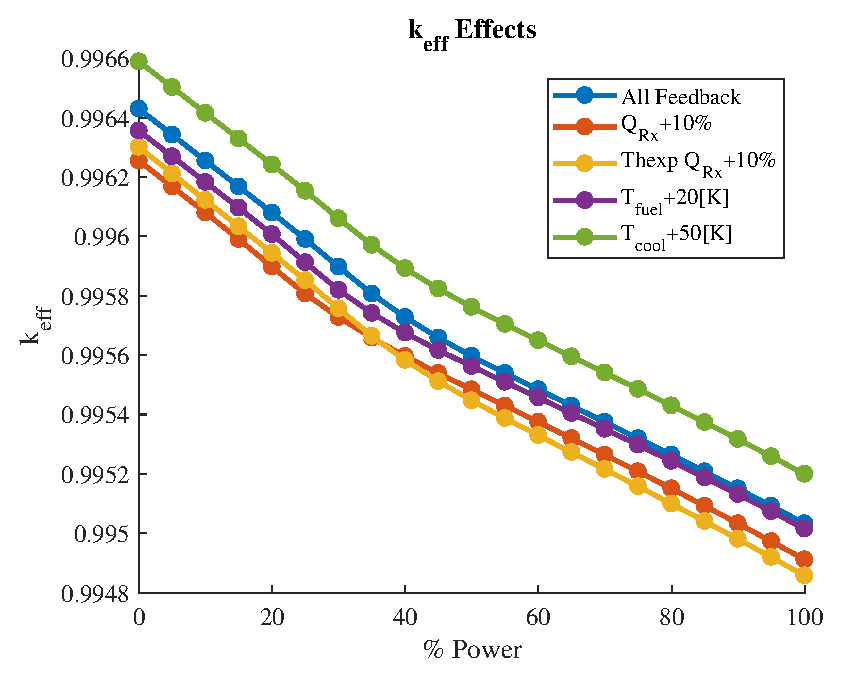
\includegraphics[width=0.7\textwidth]{keff_effects}
    \caption{Feedback Effects on $\keff$.}
    \label{fig:keff_effects}
  \end{figure}

  \begin{figure}
    \centering
    \subfloat[Power Reactivity Coefficient.]{
      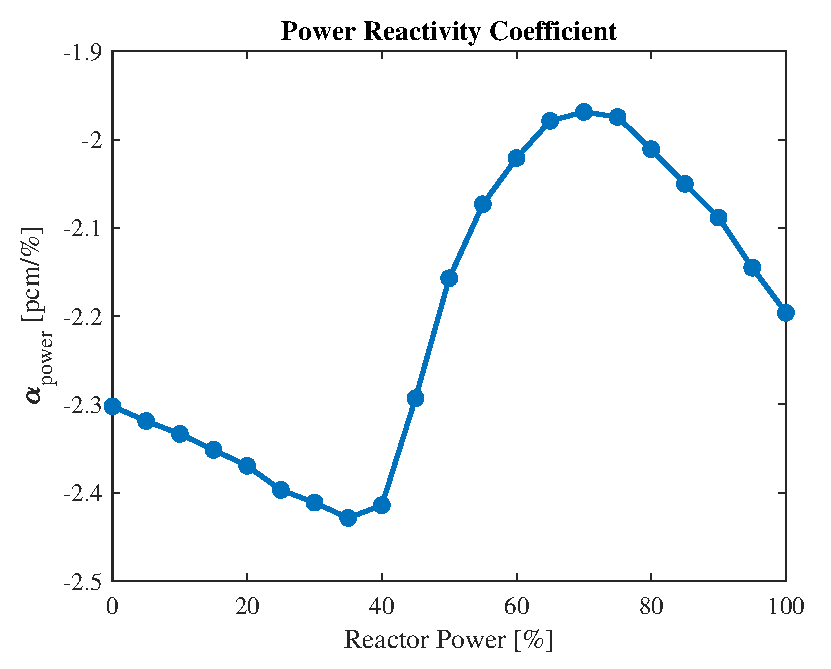
\includegraphics[width=0.5\textwidth]{alpha_power}
      \label{fig:power_reactivity_coefficient}}
    \hspace*{\fill}
    \subfloat[Thermal Expansion Reactivity Coefficient.]{
      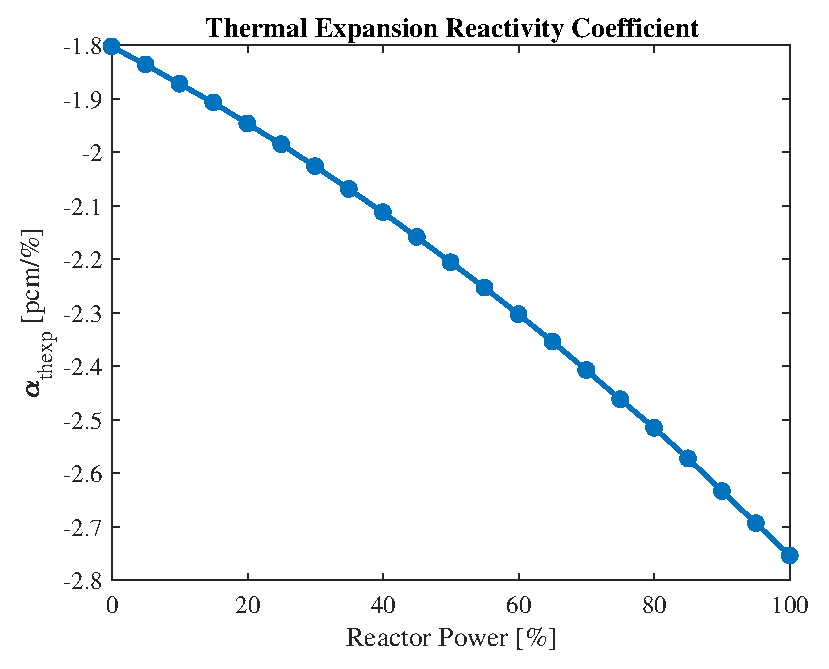
\includegraphics[width=0.5\textwidth]{alpha_thexp}
      \label{fig:thermal_expansion_reactivity_coefficient}}
    \vspace{\baselineskip}
    \subfloat[Doppler Reactivity Coefficient.]{
      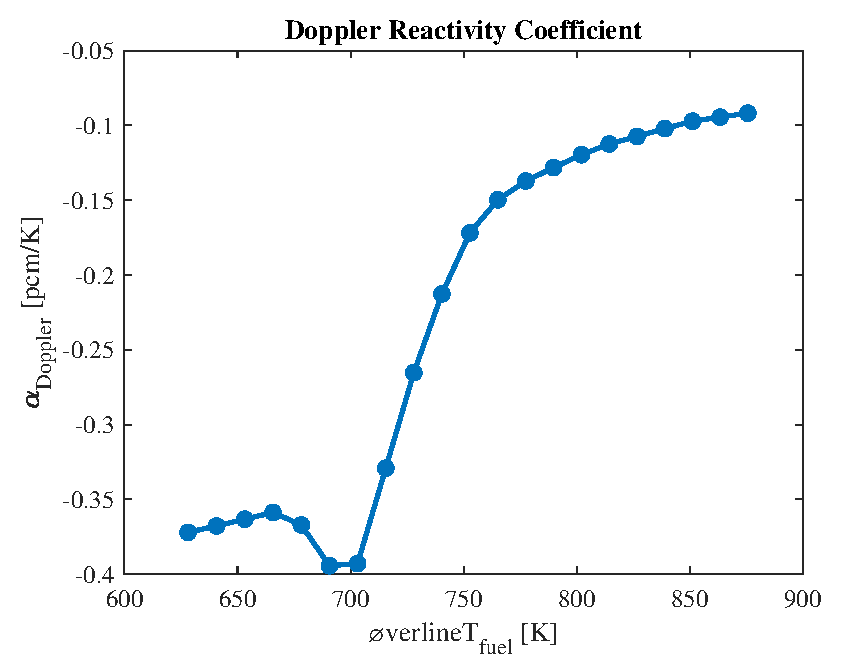
\includegraphics[width=0.5\textwidth]{alpha_fuel}
      \label{fig:doppler_reactivity_coefficient}}
    \hspace*{\fill}
    \subfloat[Coolant Temperature Reactivity Coefficient.]{
      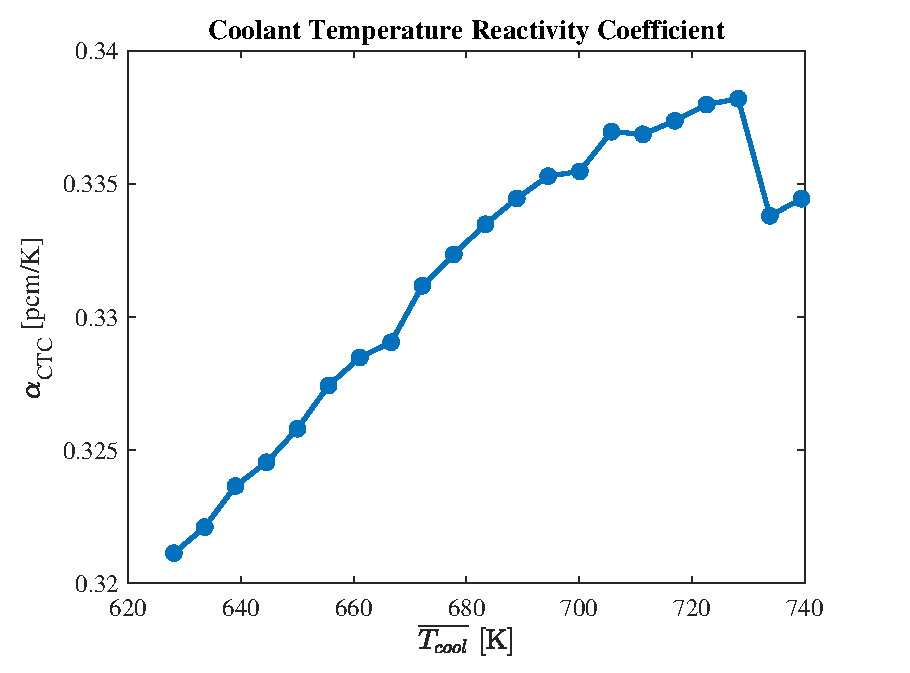
\includegraphics[width=0.5\textwidth]{alpha_cool}
      \label{fig:coolant_temperature_reactivity_coefficient}}
    \caption{\gls{abr} Reactivity Coefficients.}
    \label{fig:abr_reactivity_coefficients}
  \end{figure}

  Multiphysics effects are summarized in \tref{tab:multiphysics_worths}. To
  separate the contributions of thermal hydraulics and thermal expansion, the
  reactor was simulated using only the thermal expansion model and using both
  thermal expansion and thermal hydraulics models.  The data in
  \tref{tab:multiphysics_worths} indicates a power defect of
  $-589.49~\units{pcm}$.  This power defect is slightly lower than other
  \glspl{sfr}, but this reactor was designed for steady-state neutronics
  calculations, not multiphysics simulations. The majority of the power defect,
  $-559.64~\units{pcm}$, is attributed to thermal expansion effects.
  The remaining $-29.85~\units{pcm}$ is attributed to thermal hydraulics and 
  cross section feedback effects. This number is a bit deceiving as there is a
  cancellation of errors occurring. The Doppler reactivity coefficient and
  \gls{ctc}, as plotted in \fref{fig:doppler_reactivity_coefficient} and
  \fref{fig:coolant_temperature_reactivity_coefficient} respectively, are shown
  to have similar magnitude and opposite signs. For the \gls{abr} design, these
  coefficients are similar in magnitude but other reactors may not have such a
  cancellation. Therefore, the thermal hydraulics effects remain important for
  accurate simulation of a general fast reactor.

  \begin{table}
    \caption{Reactivity Worths of Multiphysics Effects.}
    \label{tab:multiphysics_worths}
    \begin{center}
      \begin{tabular}{cccc}
        \toprule
        Case & $\keff$ & $\rho~\units{pcm}$ & Incremental Worth $\units{pcm}$ \\
        \midrule
        No Feedback & 0.999808 & & \\
        \addlinespace[0.1in]
        Only Thermal Expansion & 0.994246 & -559.64  & -559.64 \\
        \addlinespace[0.1in]
        \shortstack{Thermal Hydraulics \\and Thermal Expansion} & 0.993950 &
          -589.49 & -29.85 \\
        \bottomrule
      \end{tabular}
    \end{center}
  \end{table}
